%% The following is a directive for TeXShop to indicate the main file
%%!TEX root = diss.tex

\chapter{A Description of 3D Reconstruction}
\label{ch:3DRecon_Desc}
In Chapter~\ref{ch:3DRecon_ProbSpace}, we introduced a problem space for 3D reconstruction, which provides a new perspective to understanding algorithms without delving into algorithm details. However, it is not sufficient to merely have a problem space when it comes to creating an interface for 3D reconstruction. It provides little in terms of describing problem conditions that we are interested in solving. There are two key components that are needed in order to provide a consistent description: a model which addresses \textit{what} to describe, \ie which property is included or excluded in the model, and corresponding representations addressing \textit{how} to describe the components of a model, \ie what characteristics of a property should be of interest. The first issue has already been somewhat addressed in Chapter~\ref{ch:3DRecon_ProbSpace} with the well-defined problem space. Specifically, we can use a subset of properties of the problem space as the components of the model. However, the second issue has yet to be addressed. We have not discussed which aspect of a property is crucial to problem solving, and how it is measured or estimated. Besides, it is pointless to discuss the estimation of property parameter without determining the corresponding representation beforehand. Thus, it is practically impossible to provide a consistent description without a model and corresponding representations. Here is a concrete example to further stress the importance of model and representations: how to describe a porcelain vase? First and foremost, we need to decide which properties to describe. We use surface `texture' as an example. Next we need to address how this property, `texture' in this example, is represented, \ie what characteristics of the property is used to measure the strength of `texture'. We can choose the scale of texel (texture element), or randomness of texel as representation of texture. Otherwise, it make no sense to quantify a property before determining the corresponding representation. Thus, this chapter addresses these two issues: first, we propose a model consisting of a subset of properties from the problem space. We recognize that it is practically impossible to achieve an exhaustive description, and the scope of description is determined by the scope of the problem space. For instance, sub-surface scattering property should not be included in the description since it is omitted in the problem space as well. Secondly, we need to determine the representation of each property. Each property might have multiple facets that are essential to problem solving. For instance, when we talk about texture, some important features include randomness of texture, scale of texel, magnitude and orientation of texture, and so on. Without determining a proper representation of the property, there is no way we can proceed to perceptually estimate the strength of the property.
% Thus, this chapter is concerned with defining an interpretable description to select an algorithm, which consists of a model and corresponding representations.

This way of thinking is not specific to our problem. Typical computer vision problems require, among other factors, a model of the problem space and appropriate representations~\cite{little1985phdthesis}. The model characterizes the relevant properties of the elements in the domain and analyze their relations. The representations describe an object's properties selected by the model to facilitate a solution of the problem. For instance, surface orientation is a part of the surface geometry model, and the corresponding representation can be surface normal or curvature. Another example is colour, which is a component of a material model, and the RGB values could be one of the representations of this property. By using this formal description consisting of a model and corresponding representations, expressing the conditions within which an algorithm works reliably becomes more well-defined. Thus, this chapter is devoted to proposing a model and representations for 3D reconstruction problem, which are the key components of the interpretable description.

In this chapter, we attempt to provide a description of the 3D reconstruction problem which allows for a well defined specification of the conditions surrounding the problem. This description abstracts away from the functional specification of \textit{how} to estimate a reconstruction. We first propose a formal definition of the 3D reconstruction problem in Appendix~\ref{sec:3DRecon_Def}. Next, Section~\ref{sec:3DRecon_Model} proposes a model to 3D reconstruction by selecting various key \textit{characteristics} of the problem space that are crucial for describing the appearance of the object. Section~\ref{sec:3DRecon_Rep} discusses corresponding representations of the proposed model. Section~\ref{sec:3DRecon_Exp} provides examples of expressing 3D reconstruction problems using the proposed model and representations. These following four layers represent the description of our accessible 3D reconstruction framework: Definition, Model, Representation, and Expression.

\section{Model}
\label{sec:3DRecon_Model}
Model and representations are fundamental for vision problem solving. Model selects characteristic properties of an object, and representations describe the model selected object properties to facilitate a solution of a class of problem. A model facilitates the representation of aspects in reality that are useful in a particular problem domain~\cite{bolles19863dpo}. There are two criteria in choosing the model: 1) the model components need to be useful for problem solving; 2) the components need to be visually or perceptually identifiable so that it is easy for users to learn to describe problem conditions using the proposed model. As discussed in Chapter~\ref{ch:RelatedWork}, visual and geometric information, such as texture, shading variations, and silhouette are critical to 3D vision algorithms. In Chapter~\ref{ch:3DRecon_ProbSpace}, we summarized key visual and geometric properties of an object that are of great importance for humans to identify and distinguish objects. It is clear that a subset of information that both vision algorithms and humans utilize overlaps, for instance, both textural and brightness information are utilized. Thus, we select a subset of properties that are used by vision algorithms as reconstruction cues, and also easily identifiable by humans as the main components of our model.

The selection of algorithm depends not only on material and shape of objects, but also on the capturing system. The lighting condition determines if certain categories of algorithms can be used. For instance, active methods needs controlled lighting condition, which typically use a light source or projector whereas passive methods work under ambient lighting. The number of vantage points determines whether a single vantage point algorithm or multiple vantage points algorithm is utilized. Lastly, the static or dynamic nature of the scene determines whether an algorithm that can dynamically update the scene is needed. The key components of the model are shown in Table~\ref{tab:3DRecon_model}.
\begin{table}[!htbp]
  \centering
  \begin{tabular}{l|l}
  \toprule
  \multirow{5}{*}{Model} 
  & Lighting \\
  & Vantage points \\
  & Nature of object or scene \\
  & Texture \\
  & Brightness \\
  & Reflectance \\
  & Roughness \\
  & Concavity \\
  \bottomrule
  \end{tabular}
  \caption{Model of the 3D reconstruction problem. Visual and geometric properties are selected from the problem space in Chapter~\ref{ch:3DRecon_ProbSpace}.}
  \label{tab:3DRecon_model}
\end{table}

% In addition to these properties, there are requirements that can be imposed to the final reconstruction result. These requirements include but not exclude:

% \begin{table}[h]
%   \centering
%   \begin{tabular}{l|*{5}{c}}
%   \hline
%   \textbf{Requirement} & Accuracy-first & Completeness-first & Orientation-first & Roughness & Concavity\\
%   \hline
%   \end{tabular}
%   \caption{Model of the 3D reconstruction problem: requirements}
%   \label{tab:3DRecon_model}
% \end{table}

\section{Representation}
\label{sec:3DRecon_Rep}
Based on the proposed model of the 3D reconstruction problem, we need to further define the representations so that the 3D reconstruction problem can be expressed using the proposed model and representations.

% We look at the \textit{cues} that are utilized by 3D reconstruction techniques and their corresponding contributing properties. In Chapter~\ref{ch:3DRecon_Taxo}, we explored a new taxonomy of 3D reconstruction based visual/geometric cues. Now we need to investigate the visual and geometric properties of the object that can affect those cues. This section is organized by the visual/geomtric cues, and the visual/geomtric properties are investigated in each section.

% \subsection{Segment and scell}
% As defined in section~\ref{sec:3DRecon_Def}, a segment is the 3D to 2D transformation of a scell. Here we discuss concrete examples of segment and scell.

% \subsubsection{Pixel and voxel}
% In the image plane, a pixel is a square of size $1\times 1$. In the matrix representation of an image $I$, a pixel is an entry of the matrix, $I(x, y)$. A voxel is a 3D regular cube, and the center of which is projected to the center of the pixel.
% \begin{figure}[h]
% \centering
% 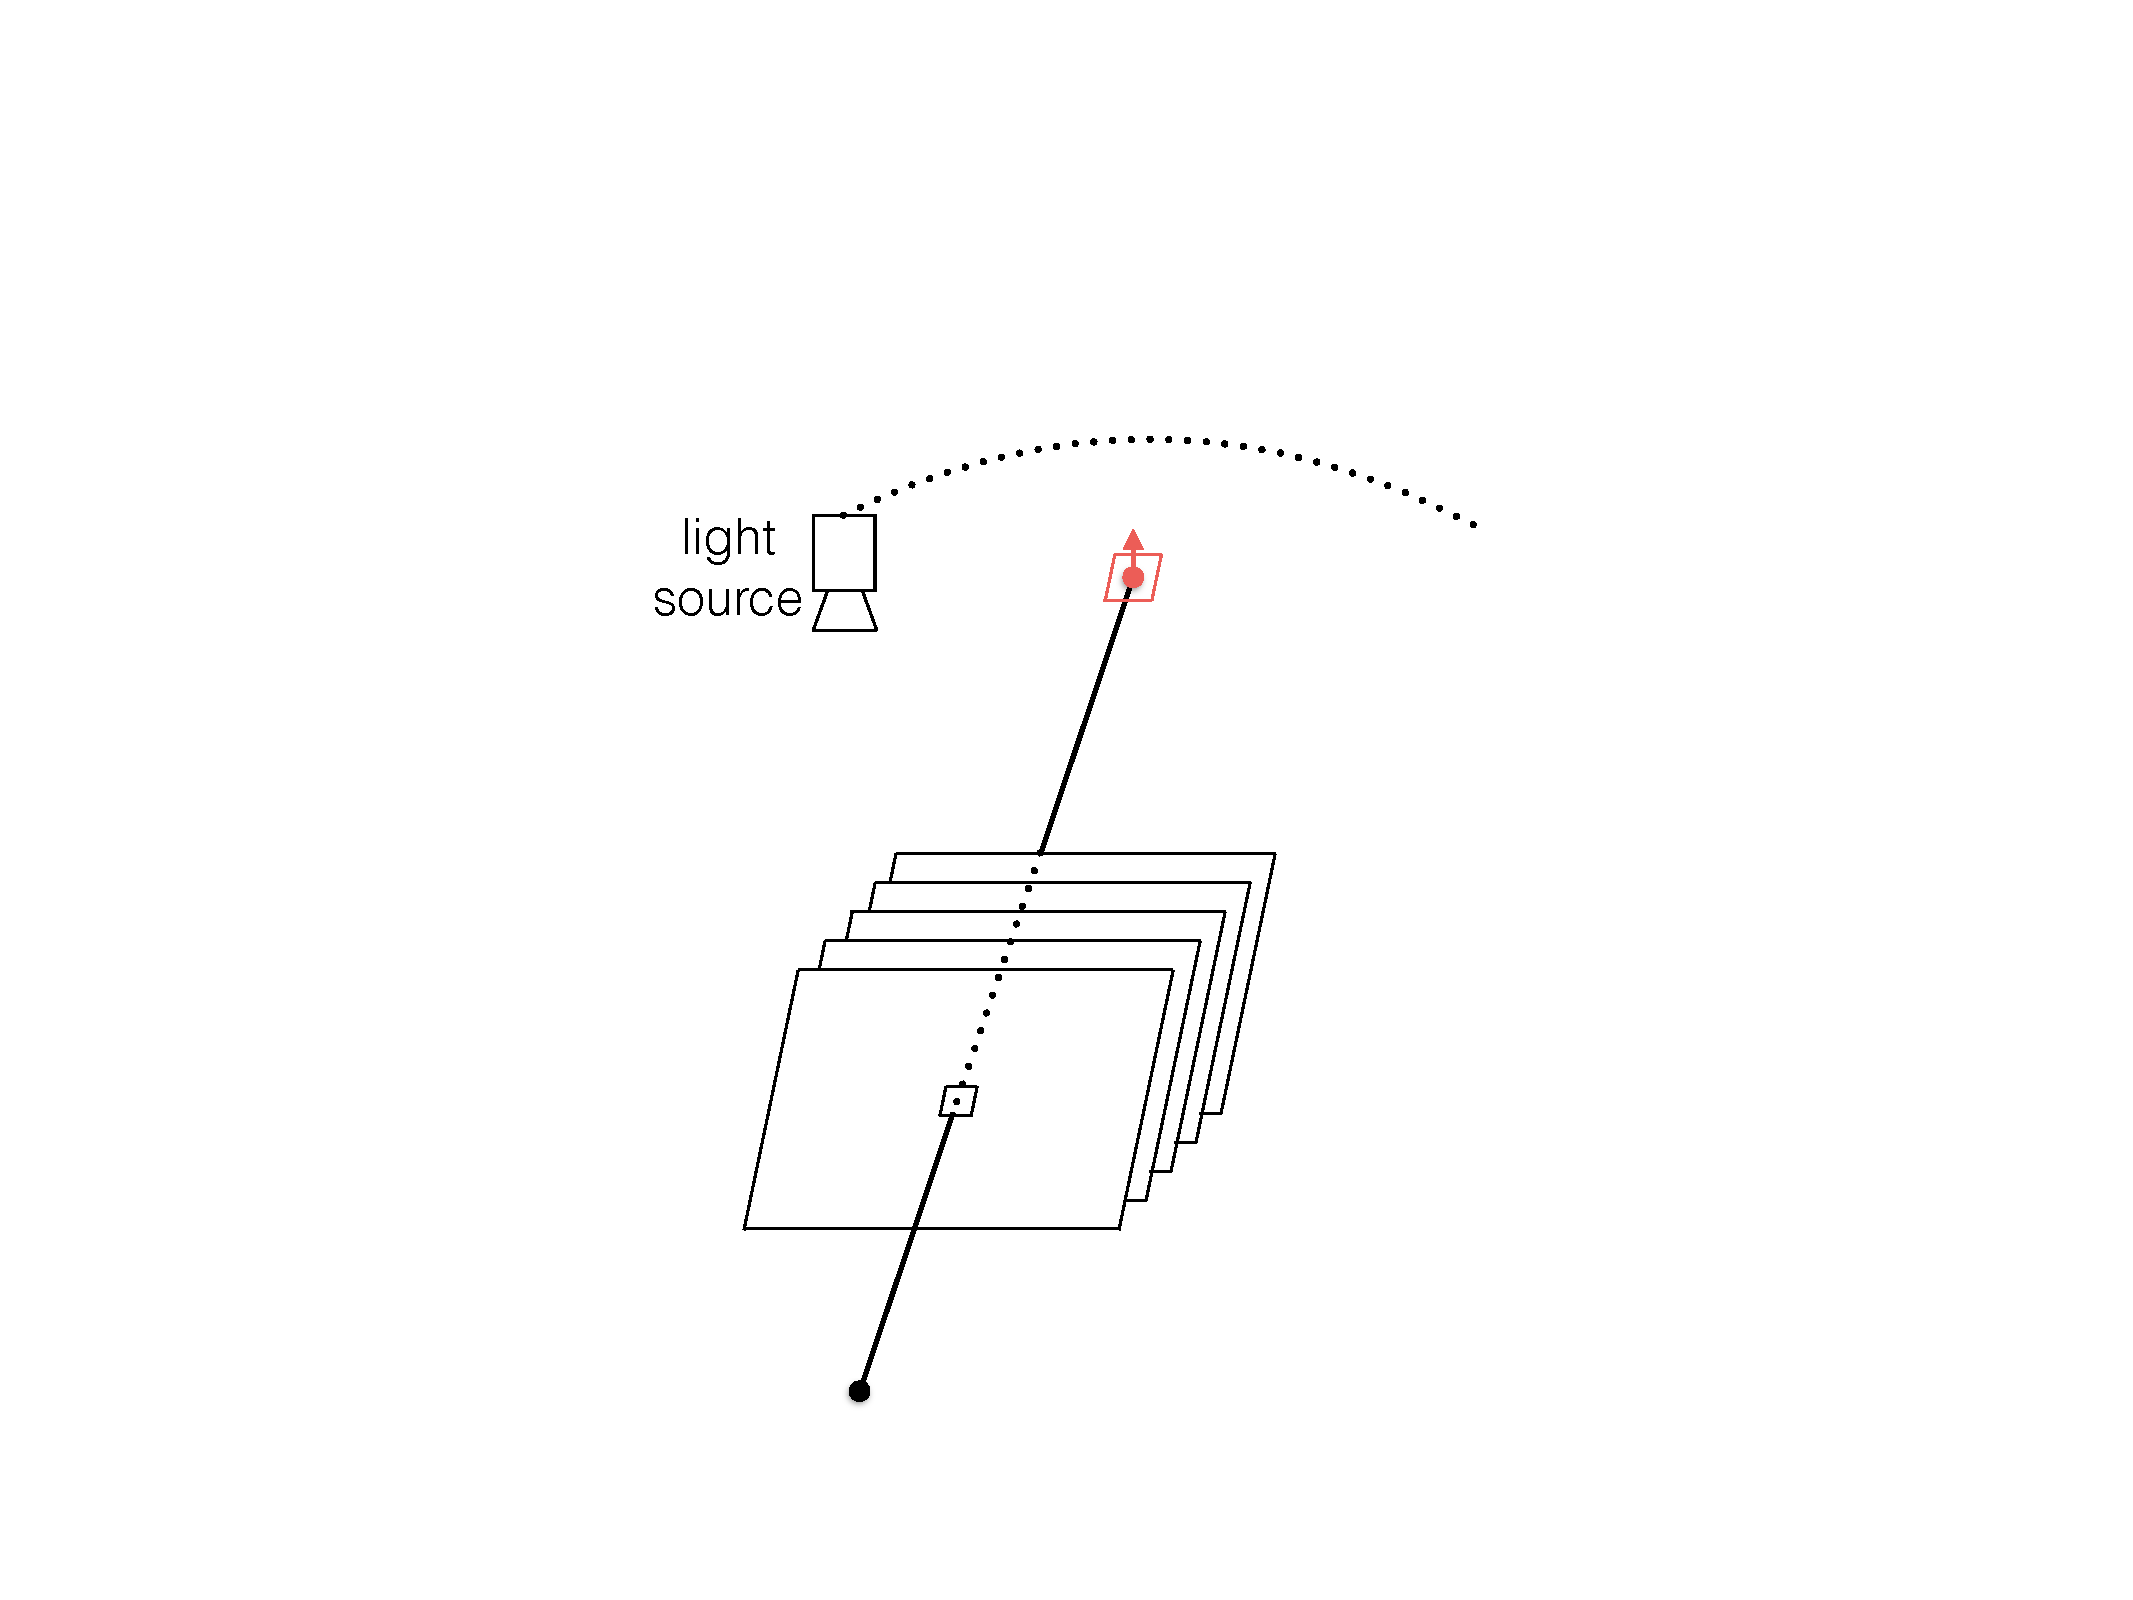
\includegraphics[width=0.5\texturewidth]{desc/pixel_voxel}
% \caption{Pixel and voxel}
% \end{figure}

% \subsubsection{Silhouette and bounding edge}


% \subsubsection{Window area and patch}
% A window area is contained in a $w\times w$ regular square, and the surface patch is a 3D point of $p\times p$ with a normal vector.
% \begin{figure}[h]
% \centering
% 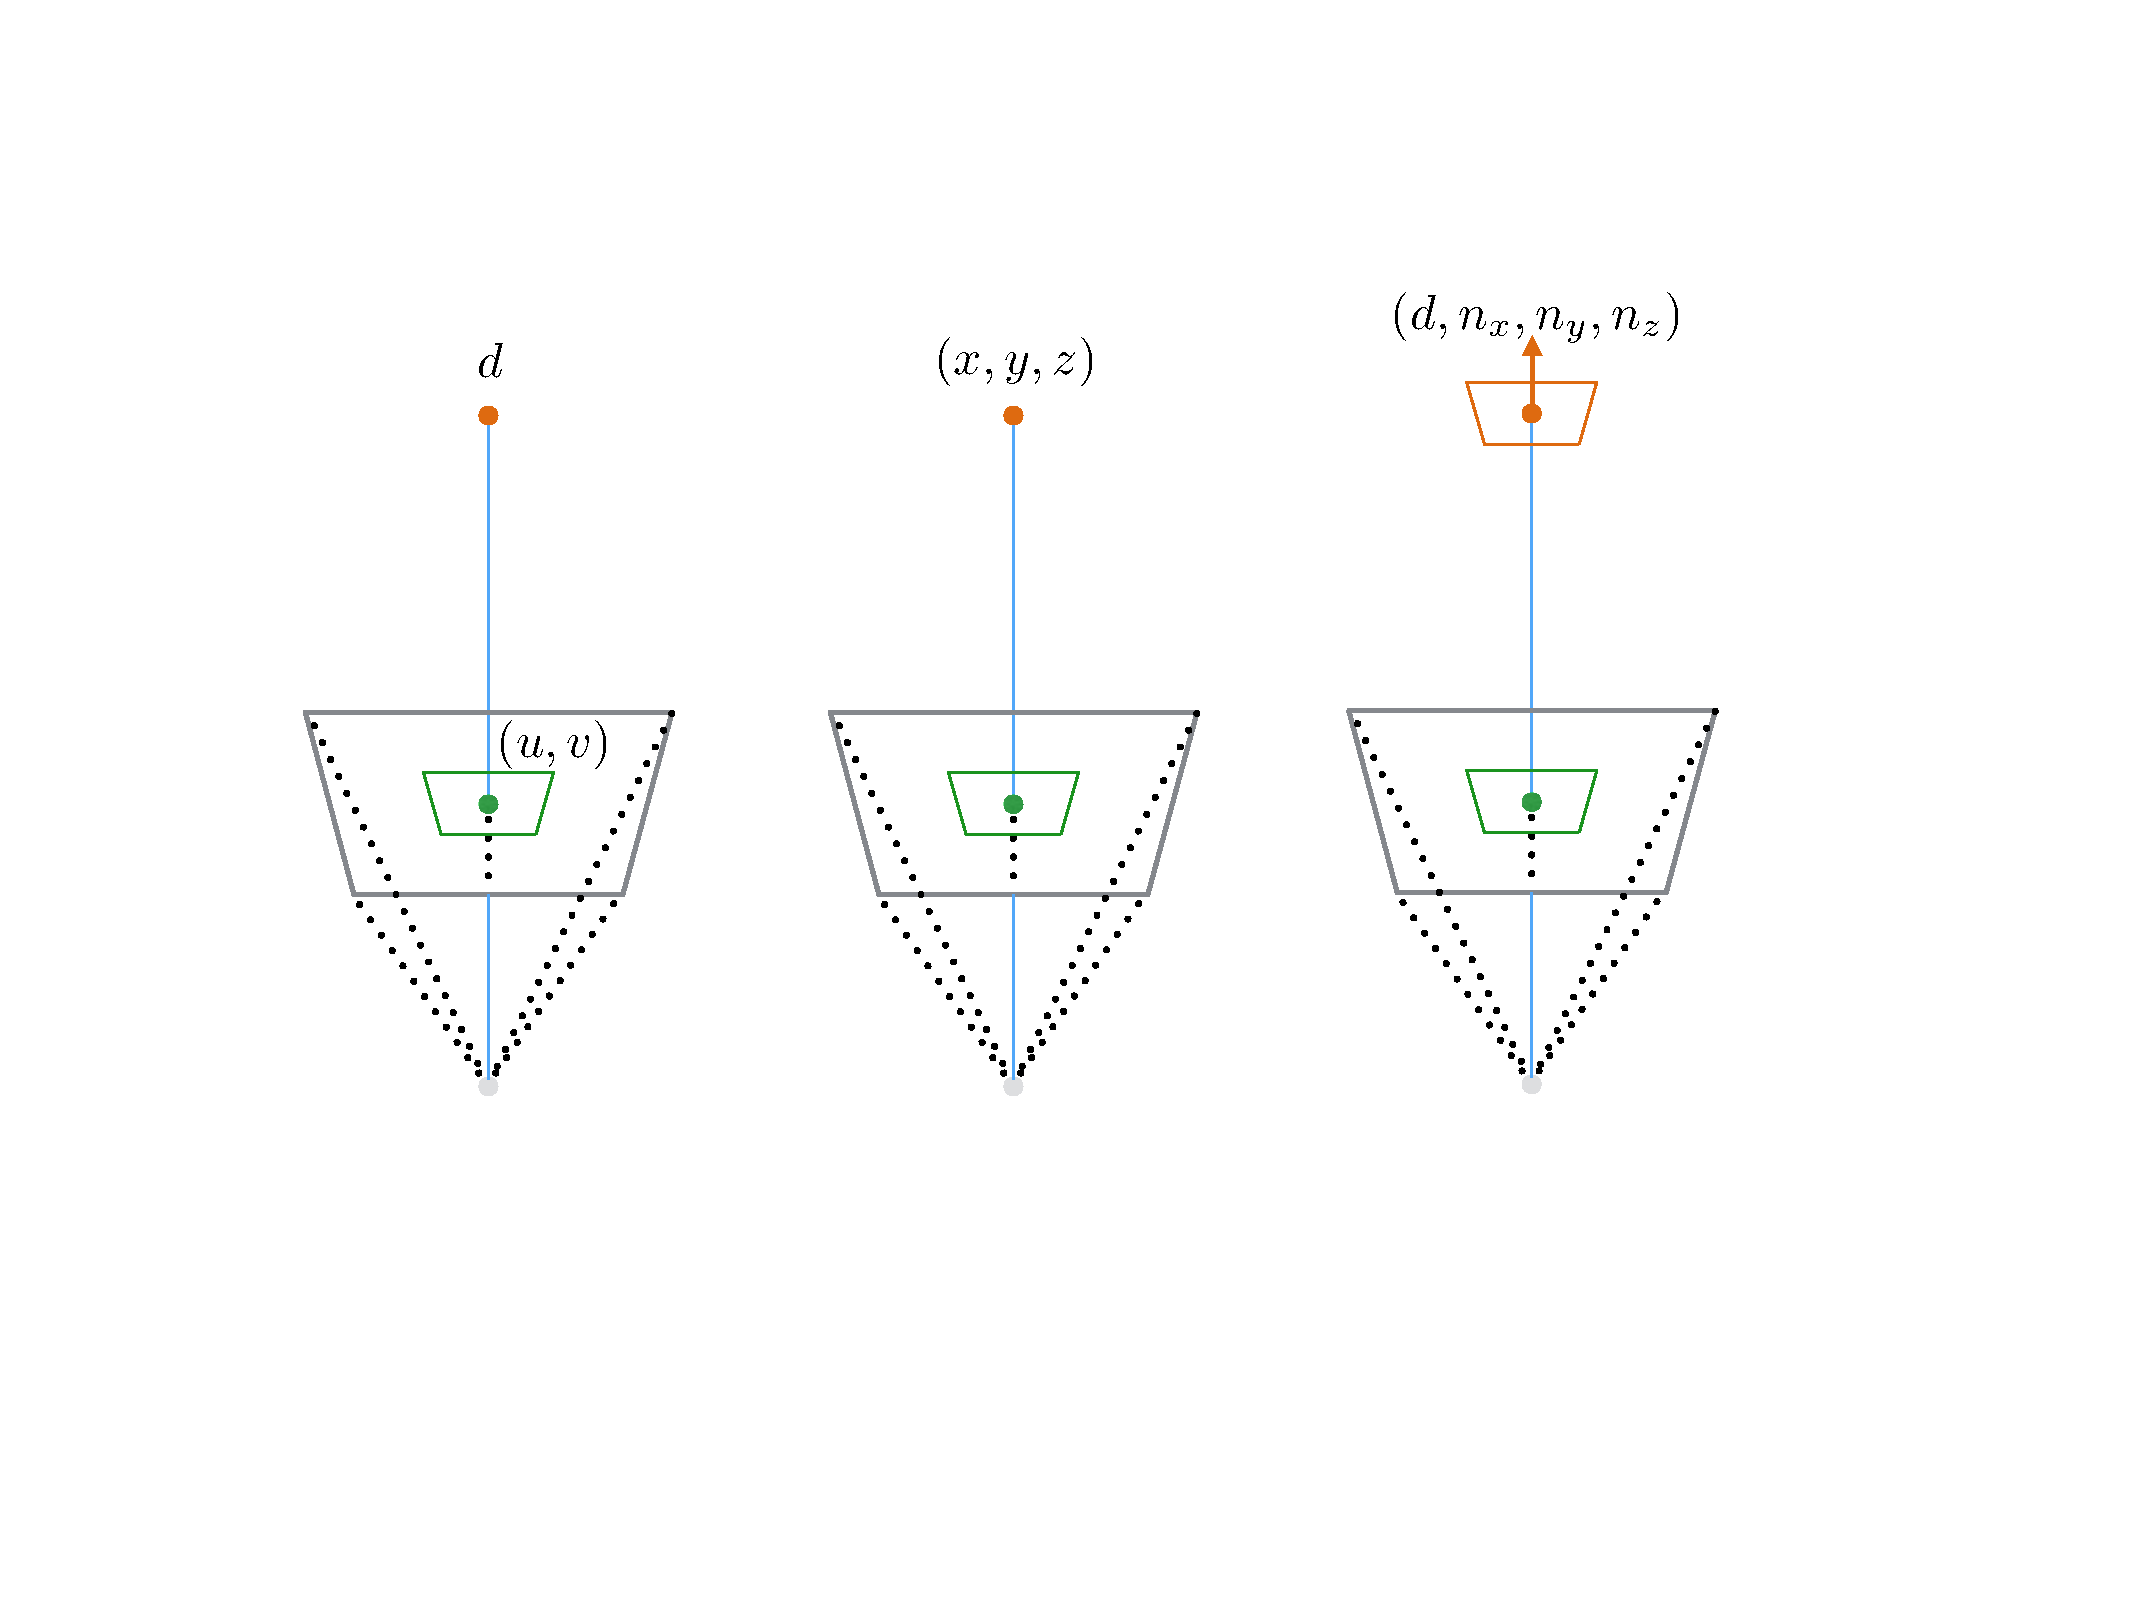
\includegraphics[width=0.8\textwidth]{desc/window_patch}
% \caption{a window area and a surface patch}
% \end{figure}

% \subsection{Cues and properties}
% As defined in Chapter~\ref{sec:3DRecon_Def}, cue is the characteristics of the segment while property is that of the scell. For each cue observed in a segment, we discuss the underlying properties that have an impact on it.
\subsection{Setup of Capturing System}
The model of the capturing system includes the lighting condition, the number of vantage points, and the nature of the object or scene. In this thesis, we use a fixed capturing system, thus the configurations of the capturing system is constant throughout the thesis, thus is omitted in the following discussions for the sake of brevity. The configuration of the capturing system is shown in Table~\ref{tab:capture_system_representation}.
\begin{table}[!htbp]
    \centering
    \begin{tabular}{lll}
        \toprule
        \textbf{Model} & \textbf{Representations} & \textbf{Value} \\
        \midrule
        \multirow{2}{*}{Nature of scene} & \tc{Static} & \\
                                         & Dynamic & \\ \cline{1-3}
        \multirow{4}{*}{Lighting} & Passive & Ambient light\\
                                  & \multirow{2}{*}{Active} & Light source\\
                                  &  & Projector\\
                                  & Mixed & \tc{Ambient\& light source\& projector} \\ \cline{1-3}
        \multirow{4}{*}{Vantage point} & Single vantage point & 1 \\
                                   & \multirow{3}{*}{Multiple vantage points} & Small ($<10$) \\
                                   &                                          & \tc{Medium ($10 - 50$)} \\
                                   &                                          & Large ($>50$) \\
        \bottomrule
    \end{tabular}
    \caption{The representations of the capturing system. The configuration of the current capturing system is label in red.}
    \label{tab:capture_system_representation}
\end{table}

\subsection{Texture}
Texture is one of the most important cues for many computer vision algorithms. It is generally divided into two categories, namely \textit{tactile} and \textit{visual} textures. Tactile textures refer to the immediate tangible feel of a surface, whereas visual textures refer to the visual impression that textures produce to the human observer, which are related to local spatial variations of simple stimuli like colour, orientation and intensity in an image. Here we focus only on visual textures, as they are more widely used in the stereo vision research. The term `texture' hereafter refers exclusively to `visual texture' unless mentioned otherwise.

Although texture is an important component in computer vision, there is no precise definition for the notion of texture itself. The main reason for this is that natural textures often exhibit separate yet contradicting properties, such as regularity versus randomness, or uniformity versus distortion, which can hardly be described in a unified manner. 
% Haralick considers a texture as an ``organized area phenomenon'' which can be decomposed into `primitives' having specific spatial distributions~\cite{haralick1979statistical}. This definition, also known as structural approach, comes directly from human visual experience of texture. These primitives are organized in a particular spatial structure indicating certain underlying placement rules. Alternatively, as Cross and Jain suggested, a texture is ``a stochastic, possibly periodic, two-dimensional image field''~\cite{cross1983markov}, which is also known as \textit{stochastic approach}.

% For s regular textures, there are two basic dimensions on which it may be described. The first dimension is for describing the primitives out of which the texture is composed, and the second dimension is for the description of the spatial dependence or interaction between the primitives of an image texture. The first property is concerned with tonal primitives and local properties, and the second dimension is concerned with the spatial organization of the tonal primitives.

There are various properties that make texture distinguishable: scale/size/granularity, orientation, homogeneity, randomness, etc. However, due to the diverse and complex nature of textures, it is a challenging task to generate a synthetic texture solely from these semantic properties, or the other way around, derive parameters from a given texture. The stereo vision community often takes a simplified approach, classifying textures into two categories, regular and stochastic, by degree of randomness. A regular texture is formed by regular tiling of easily identifiable elements (texels) organized into strong periodic patterns. A stochastic texture exhibits less noticeable elements and displays rather random patterns. Most of the real world textures are mixtures of these two categories. In this thesis, we adopt this simplification and consider \textit{texture randomness}, which is the amount of distortion in the texture. Thus, a uniform texture has low \textit{texture randomness} whereas a highly textured surface has high \textit{texture randomness}.

% Most texture synthetic research has focused on data-driven or statistical approaches. For the data-driven approach, the generated texture is not general enough whereas it's not intuitive enough for the statistical approach. Thus we turn to an approach that is more tailored to the stereo vision problem. Based on the observations from practical tests, stereo algorithms work well under the condition of non-uniform texture, even for textures caused by shadow. This is theoretically plausible as stereo vision tries to find the correspondence based on the `distinctiveness' of the texture. Therefore, as long as the surface is covered by distinct texture, it doesn't matter what the basic texture element is. Thus the most significant attributes of the texture is coverage, \ie the percent of the surface that is covered, and it's the focus of this thesis.

% Texture is formally defined as a set of texture element or \textit{texels} occuring in some regular, or repeated, or random pattern. Texture gives us information about the \textit{spatial arrangement} of the colours or intensities in an image. However, it is something that is easy to recognize, but hard to define. 

% Here we only consider visual textures, which is the result of shape and reflection. Therefore, a surface with varying reflectance property can produces a textured surface, a flat surface with fixed reflectance property under different illuminations can also achieve textured effect. Even very weak texture can be a strong cue to object reconstruction as manifested by the Middlebury `Dino' dataset.

\subsection{Brightness}
When light strikes a surface, it may be reflected, transmitted, absorbed, or scattered; usually, a combination of these effects occurs. The intensity or colour information received by a sensor is thus determined, among other factors, by the amount of light available after these interactions. We assume that all effects are local, thus global effects such as inter-reflection and transmission, among others, are omitted. This is called a \textit{local interaction model}. In order to understand the contributing factors of pixel intensity or colour, we need an in-depth understanding of reflection, \ie how light is reflected off of a surface patch, and the relation between material and intensity values. The radiometric formation of an image consists of three separate processes: \textit{light-matter interaction}, \textit{light-lens interaction}, and \textit{light-sensor interaction}, as discussed in Appendix~\ref{sec:pbv}. The conclusion is that image intensity is proportional to \textit{diffuse reflectance} (\textit{albedo}).
% Here, we consider intensity as caused solely by reflection, since this is one of the most common phenomena experienced and is the easiest to analyze. Lightness ranges from `black' to `white' in the grey scale axis, and colour is a superset of intensity, which takes into account the spectral composition of light. Both lightness and colour depend on illumination, surface normal, surface reflectance, and viewing direction.

Diffuse reflectance represents light that is refracted into the surface, scattered, partially absorbed, and re-emitted. The Lambertian diffuse model assumes that the refracted light has scattered enough that it has lost all directionality and thus the diffuse reflectance is constant. However, very few materials exhibit a Lambertian response. Many materials show a drop in grazing retro-reflection, and many others show a peak. This is strongly correlated to surface roughness --- smooth surfaces tend to have a shadowed edge, and rough surfaces tend to have a peak instead of a shadow. This grazing shadow for smooth surfaces can be explained by the Fresnel equations: at grazing angles, more energy is reflected from the surfaces and less is refracted into the surface to be diffusely re-emitted. However, diffuse models don't generally consider the effect of surface roughness on Fresnel refraction and either assume a smooth surface or ignore the Fresnel effect. In this thesis, we adopt this diffuse model that neglects surface roughness, thus the albedo is considered constant, and not affected by grazing angle and surface roughness.

In conclusion, as long as the \textit{light-sensor interaction} is considered as a linear mapping (as most vision algorithms do) or calibrated in a pre-processing step, the pixel intensity value is linearly proportional to diffuse reflectance, which is the representation we adopt for brightness.

% The reflectance of light also depends on the incident direction. Specifically, light that lands on a surface at a grazing angle will be much more likely to reflect, see Figure~\ref{fig:alb_ang}. We take into account the Fresnel effect in the synthetic stage, thus we consider the albedo with small incident angle.
% \begin{figure}[h]
% \centering
% 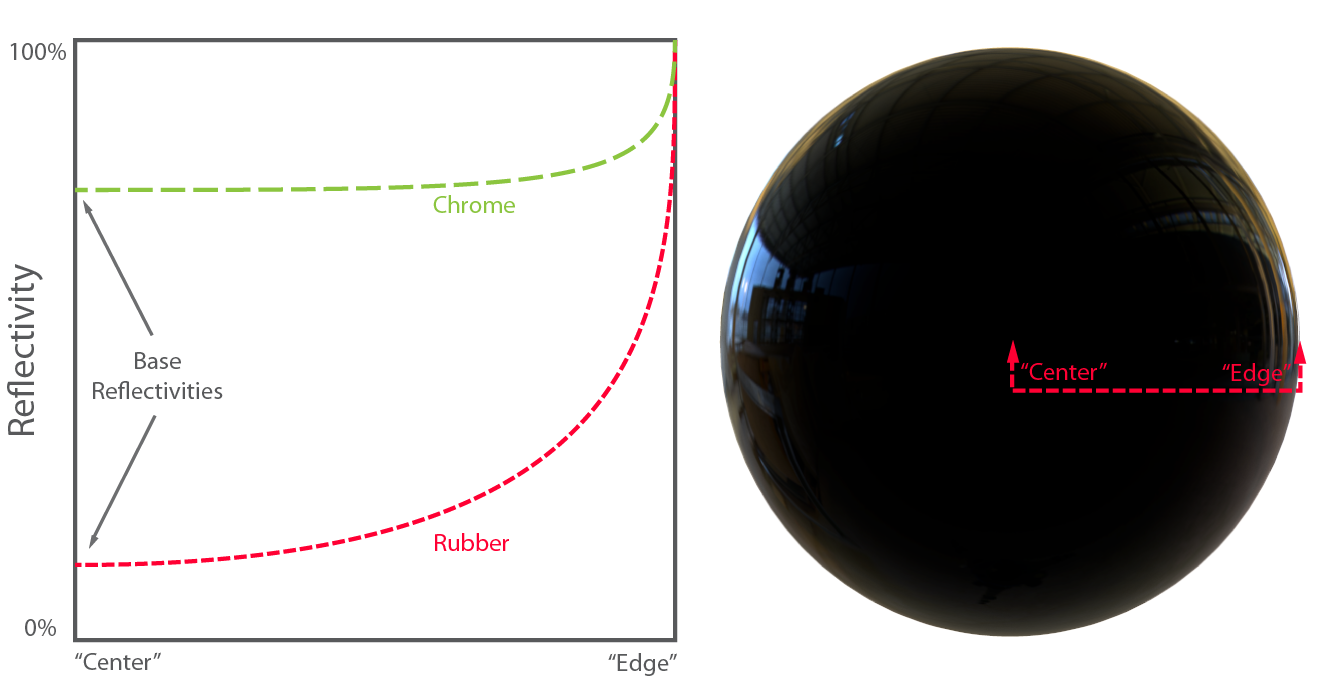
\includegraphics[width=0.5\textwidth]{desc/reflectance_angle}
% \label{fig:alb_ang}
% % \caption{Spectral reflectance curves for aluminium (Al), silver (Ag), and gold (Au) metal mirrors at normal incidence.}
% \end{figure}

\subsection{Specularity}
Specular surfaces reflect light in nearly a single direction when microscopic surface irregularities are small compared to light wavelength, and no subsurface scattering is present~\cite{nayar1989surface}. Unlike diffuse reflections, where we experience the brightness and colour of an object, specular reflections carry information about the structure, intensity, and spectral content of the illumination field. In other words, specular reflection is simply an image of the environment, or the illumination field, distorted by the geometry of the reflecting surface. For instance, the specular sphere in Figure~\ref{fig:spec_ref} shows a distorted image of the environment instead of the underlying surface colour. A purely specular surface is a mirror, which is rare in nature. Most natural materials exhibit a mixture of specular and diffuse reflections. We use the microfacet model as the reflectance model in this thesis, which is discussed in Appendix~\ref{sec:microfacet_model}. Thus the amount of specular component is determined by the \textit{Fresnel reflectance}, also named \textit{specular reflectance}.
% A commonly used model treats mixed reflectance as a weighted combination of diffuse and specular component. Thus the ratio of incident light that is specularly reflected is considered as the representation of sepcularity, with 0 being completely diffuse, and 1 being completely specular (mirror like)
\begin{figure}[!htbp]
\centering
\begin{tabular}{cc}
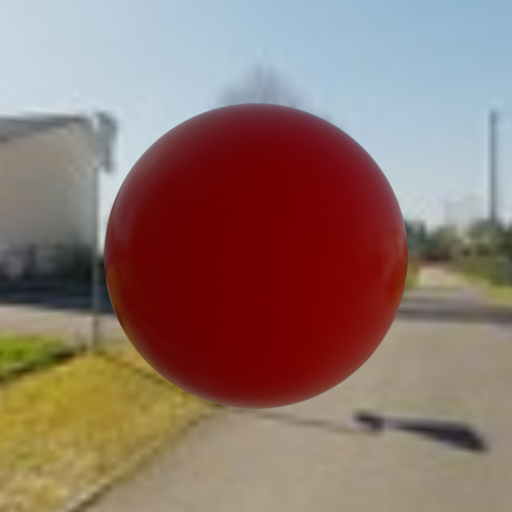
\includegraphics[width=0.2\textwidth]{desc/sphere_diffuse}&
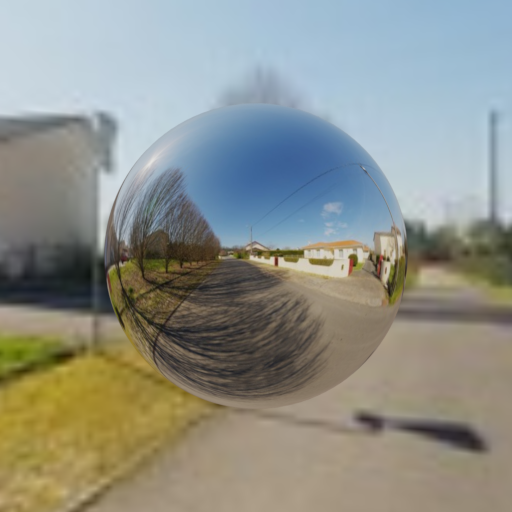
\includegraphics[width=0.2\textwidth]{desc/sphere_specular}\\
(a) & (b)\\
\end{tabular}
\caption{(a). A \textbf{red} diffuse sphere; (b). a \textbf{red} specular sphere. The surface reflects light in a mirror-like way, showing a distorted environment. Since no diffuse reflection exists, the colour of the surface is no longer visible.}
\label{fig:spec_ref}
\end{figure}

The Fresnel reflectance is the fraction of incoming light that is reflected (as opposed to refracted) from an optically flat surface of a given substance. It varies based on the light direction and the surface (in this case microfacet) normal. Fresnel reflectance tells us how much of the light hitting the relevant microfacets (the ones facing in the half-angle direction) is reflected. Fresnel reflectance depends on refraction index (in other words, what the object is made of) and the incoming light angle (which is plotted here on the x-axis), as shown in Figure~\ref{fig:fresnel_reflectance}. As the angle increases, the Fresnel reflectance barely changes for the first 45 degrees; afterwards it starts changing, first slowly up to about 75 degrees, and then for very glancing angles, it rapidly goes to $100\%$ at all wavelengths. Since the Fresnel reflectance stays close to the value for $0^\circ$ over most of the range, we can think of this value $F(0^\circ)$ as the \textit{characteristic specular reflectance} of the material. This value has all the properties of what is typically thought of as a ``colour'' - it is composed of RGB values between 0 and 1, and it is a measure of selective reflectance of light. For this reason, we will also refer to this value as the \textit{specular colour} of the surface, denoted as $\mathbf{c}_{spec}$. We choose specular reflectance as the representation of specularity.
\begin{figure*}[!htbp]
\centering
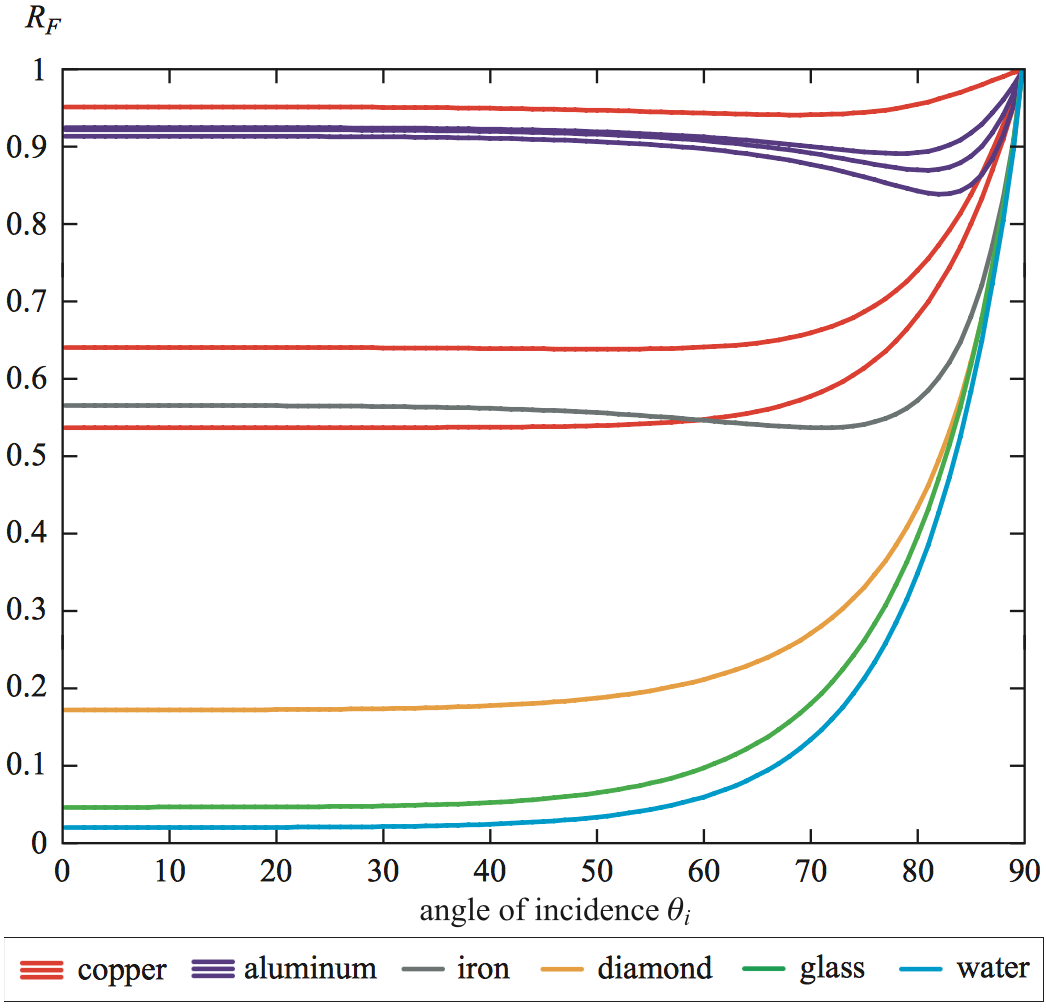
\includegraphics[width=0.55\textwidth]{desc/fresnel_reflectance.png}
\caption{Fresnel reflectance for external reflection from a variety of substances. Since copper and aluminum have significant variation in their reflectance over the visible spectrum, their reflectance is shown as three separate curves for R, G, and B. Copper's R curve is highest, followed by G, and finally B (thus its reddish colour). Aluminum's B curve is highest, followed by G, and finally R. (Image from ``Real-Time Rendering, 3rd edition'', \textcopyright 2008 A K Peters, by permission)}
\label{fig:fresnel_reflectance}
\end{figure*}

\subsection{Roughness}
Roughness, which refers to the microscopic shape characteristics of a surface, contributes to the way in which light is reflected off of a surface. A smooth surface may reflect incident light in a single direction, while a rough surface may scatter the light in various directions. Thus, variations in microscopic surface geometry can cause specular reflections to be scattered, blurring the image of the environment in an amount proportional to surface roughness. We need prior knowledge of the microscopic surface irregularities, or a model of the surface itself, to determine the reflection of incident light.

Possible surface models are divided into 2 categories: surfaces with exact known profiles and surfaces with random irregularities. An exact profile may be determined by measuring the height at each point on the surface by means of a sensor such as the stylus profilometer. This method tends to be cumbersome and impractical, hence, it is more reasonable to model the surface as a random process, where it is described by a statistical distribution of either its height above a certain mean level, or its slope with respect to its mean (macroscopic) slope. We use the second statistical approach as the representation of roughness.

% \textit{Height Distribution Model} The height coordinate of the surface is expressed as random function of the coordinates $x$ and $y$.
% \begin{figure}[h]
% \centering
% \includegraphics[width=0.5\textwidth]{desc/surface_representation_1}
% \caption{Surface height distribution model}
% \end{figure}

% The shape of the surface is determined by the probability distribution of $h$. For instance, let $h$ be normally distributed, with mean value $\bar{h}=0$ and standard deviation $\sigma_h$. Then, the distribution of $h$ is given by:
% $$
% p_h(h)=\frac{1}{\sqrt{2\pi}\sigma_h}e^{-\frac{h^2}{2\sigma_h^2}}
% $$

% The $\sigma_h$ is the root-mean-square of $h$ and represents the roughness of the surface. The surface is not uniquely described by the distribution of $h$, as it does not tell us anything about the distance between the hills and valleys of the surface.

% The surfaces below have the same height distribution function, i.e., the same mean value and standard deviation. However, they don't resemble each other in appearance.
% \begin{figure}[h]
% \centering
% \includegraphics[width=8cm]{desc/same_mean_sd}
% \caption{Surface height distribution model}
% \end{figure}

% An autocorrelation coefficient $C(\tau)$ is introduced, that determines the correlation (or lack of independence) between the random values assumed by the height $h$ at two surface points $(x_1, y_1)$ and $(x_2, y_2)$, separated by a distance $\tau$. The autocorrelation coefficient can be:
% $$
% C(\tau)=e^{-\frac{\tau^2}{T^2}}
% $$

% where $T$ is the *correlation distance*. Therefore, the above surfaces have small and large correlation distances respectively.

% \subsubsection{Slope Distribution Model}
% We can think of a surface as a collection of planar micro-facets. A large set of micro-facets constitutes an infinitesimal surface patch that has a mean surface orientation $\vec{n}$. Each micro-facet has its own orientation, which may deviate from the mean surface orientation by an angle $\alpha$.
% \begin{figure}[h]
% \centering
% 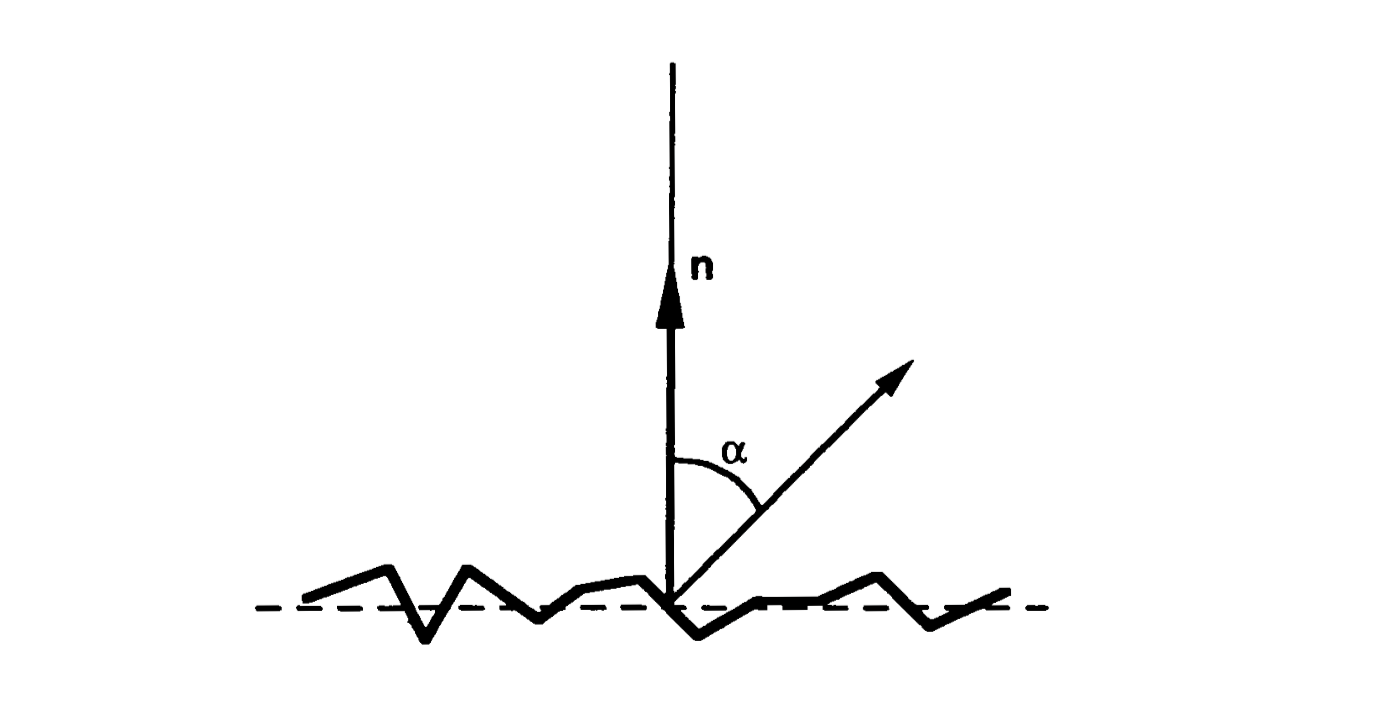
\includegraphics[width=0.7\textwidth]{desc/surface_representation_2}
% \caption{Surface Slope Distribution Model}
% \end{figure}

% We will use the parameter $\alpha$ to represent the slope of individual facets. Surfaces can be modeled by a statistical distribution of the micro-facet slopes. If the surface is isotropic, the probability distribution of the micro-facet slopes can be assumed as rotationally symmetric w.r.t the mean surface normal $\vec{n}$.  Therefore, facet slopes can be described by a one-dimensional probability distribution function. For instance, the surface may be modeled by assuming a normal distribution for the facet slope $\alpha$, with mean value $\bar{\alpha}=0$ and standard deviation $\sigma_\alpha$, where the larger $\sigma_\alpha$ can be used to model rougher surfaces:
% $$
% p_\alpha(\alpha)=\frac{1}{\sqrt{2\pi}\sigma_\alpha}e^{-\frac{\alpha^2}{2\sigma_\alpha^2}}
% $$

% The surface model is determined by a single parameter $\sigma_\alpha$ While autocorrelation coefficient is important, the concept of slope correlation is more difficult to interpret and is not that useful in the generation of surface, which results in a weaker model compared to the height model. However, slope distribution model is popular in the analysis of surface reflection, as the scattering of light rays is dependent on the local slope of the surface and not the local height of the surface.

% surface roughness will affect the fresnel and specularity

% \subsection{Concavity}
% Concavity can be measured by \textit{surface curvature}, which is defined as the inverse of the radius of a tangentially intersecting circle/sphere. We include concavity in our model for the sake of completeness. However, we decide to omit this property in the following discussion since it will introduce global light transport including cast shadow and inter-reflection, and so on, which violates our assumption of \textbf{local interaction model}. Global light transport can severely worsen the accuracy of active methods. Besides, methods that utilize silhouette information may also fail to reconstruct concavities since concavity is invisible in the silhouette images.

In conclusion, the proposed model and representation of 3D reconstruction can be summarized in Table~\ref{tab:3DRecon_model_repre}.
\begin{table}[!htbp]
  \centering
  \begin{tabular}{l|l}
  \toprule
  \textbf{Model} & \textbf{Representation}\\
  \midrule
  Nature of scene & \textit{Static} \\
  Lighting & \textit{Mixed: ambient, projector, light sources} \\
  Vantage point & \textit{Medium: 10 - 50} \\
  Texture & \textit{Texture randomness}\\
  Lightness & \textit{Diffuse reflectance}\\
  Specularity & \textit{Specular (Fresnel) reflectance}\\
  Roughness & \textit{Distribution of microfacet normal}\\
  % Concavity & \textit{Surface curvature}\\
  \bottomrule
  \end{tabular}
  \caption{A Model and corresponding representations of the 3D reconstruction problem.}
  \label{tab:3DRecon_model_repre}
\end{table}

\section{Expression}
\label{sec:3DRecon_Exp}
In this section, we discuss the expression of 3D reconstruction problems using the proposed model and representations, as shown in Table~\ref{tab:3DRecon_model_repre}. There are two related issues that need to be addressed: 1) how intuitive is the proposed model for humans to describe problem conditions; 2) how can a user estimate the parameters of properties. We first address the issue of property perception in Section~\ref{sec:prop_percept}. We can show that it is intuitive for humans to perceptually identify materials and estimate material properties. Next, we will use the proposed description to express the four problem conditions proposed in Chapter~\ref{ch:3DRecon_ProbSpace}.

\subsection{Perception of Properties}
\label{sec:prop_percept}
Different materials can be visually distinguished because they structure light in a particular, characteristic way. The way light is structured depends heavily on the shape of object, reflective and transmittive properties of material, and illumination field. This process is called the `forward optics' (image formation) process. The material perception problem is, in some sense, the `inverse optics' problem: determining what combination of surface geometry, surface material, and illumination field generated a given image~\cite{anderson2011visual}. Thus, in order to recover the reflectance properties of materials, the visual system must somehow disentangle the contributions of the illumination field and geometry. This is arguably the central problem of material perception, though the answer is currently far from clear~\cite{anderson2011visual}. But our intuition and many empirical studies support the view that humans are exceptional at material perception.

Everyday experience suggests that human's visual system are extremely good at estimating material properties. We can effortlessly distinguish numerous different categories of material: textiles, stones, liquids, foodstuffs, and so on, and can recognize many specific materials within each class such as silk, wool and cotton~\cite{fleming2014visual}. Besides, being able to visually distinguish between materials and infer their properties by sight, is invaluable for many tasks. For instance, when determining edibility, we can make subtle visual judgments of material properties to determine whether fruit is ripe, whether soup has been left to go cold or whether bread is going stale~\cite{fleming2014visual}. There are numerous experimental evidences to support this intuition. For example, \citeauthor{sharan2009material} have shown that subjects can identify a wide range of materials from photographs even with brief presentations~\cite{sharan2009material}. \citeauthor{fleming2013perceptual} showed subjects photographs of materials from different categories and asked them to rate various subjective qualities, such as hardness, glossiness and prettiness~\cite{fleming2013perceptual}. Even though subjects were not explicitly informed that the samples belonged to different classes, the subjective ratings of the individual samples were systematically clustered into categories, suggesting that subjects could theoretically classify materials through visual judgments of their properties.

There have been some empirical studies focused on visual estimation of specific properties of materials, such as glossiness, translucency or surface roughness. For instance, on the topic of glossiness, \citeauthor{nishida1998use} showed that subjects can judge the specular reflectance of computer simulated glossy surfaces~\cite{nishida1998use}, and \citeauthor{fleming2003real} showed that this ability generalizes across differences in lighting, as long as the illumination has statistical structure that is typical of the natural environment~\cite{fleming2003real}. \citeauthor{fleming2014visual} argued that the visual system does not actually estimate physical parameters of materials and objects, for instance, parameters of a reflectance model. Instead the brain is remarkably adept at building `statistical generative models' that capture the natural degrees of variation in appearance between samples~\cite{fleming2014visual}. Though there is currently no universally accepted theory on visual perception of material, both our intuition and empirical results do suggest that human are exceptionally good at `estimating' material properties.

Despite its subjective ease, material perception still poses the visual system with some unique and significant challenges, because a given material can take on many different appearances depending on the lighting, viewpoint and shape. Thus, we provide a \textit{generative} approach to visual perception: a simulation software is used to generate images of a synthetic object with varied property settings to aid the estimation of properties. The user can choose an illumination field and object shape that is closest to the real-world enviriontment and object. Then this ``trial-and-error'' approach is used to estimate parameters of properties. More specifically, the user would change the value of each property and see if the rendered result resembles the real object. A similar approach can be found in~\cite{Berkiten:2016:ARB} where \citeauthor{Berkiten:2016:ARB} used a synthetic dataset to find the contributing factors of various Photometric Stereo algorithms. We demonstrate this approach using the following example shown in Figure~\ref{fig:prop_estimate}:  the brightness of the object is controlled by the albedo value, which is determined by the value channel of HSV colour space. To determine the specularity and roughness of the object, we experiment with varying parameters to get the most realistic image.
\begin{figure}[!htbp]
\centering
\begin{tabular}{*{4}{p{2.5cm}}}
  \includegraphics[width=0.2\textwidth]{desc/desc_vase.pdf}&
  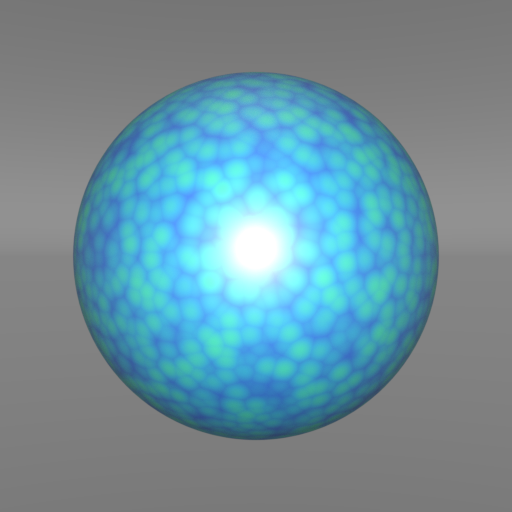
\includegraphics[width=0.2\textwidth]{interp/ui/ui_sphere.png}&
  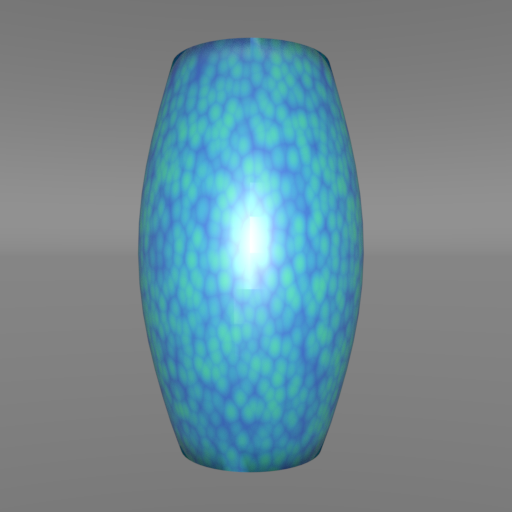
\includegraphics[width=0.2\textwidth]{interp/ui/ui_vase.png}&
  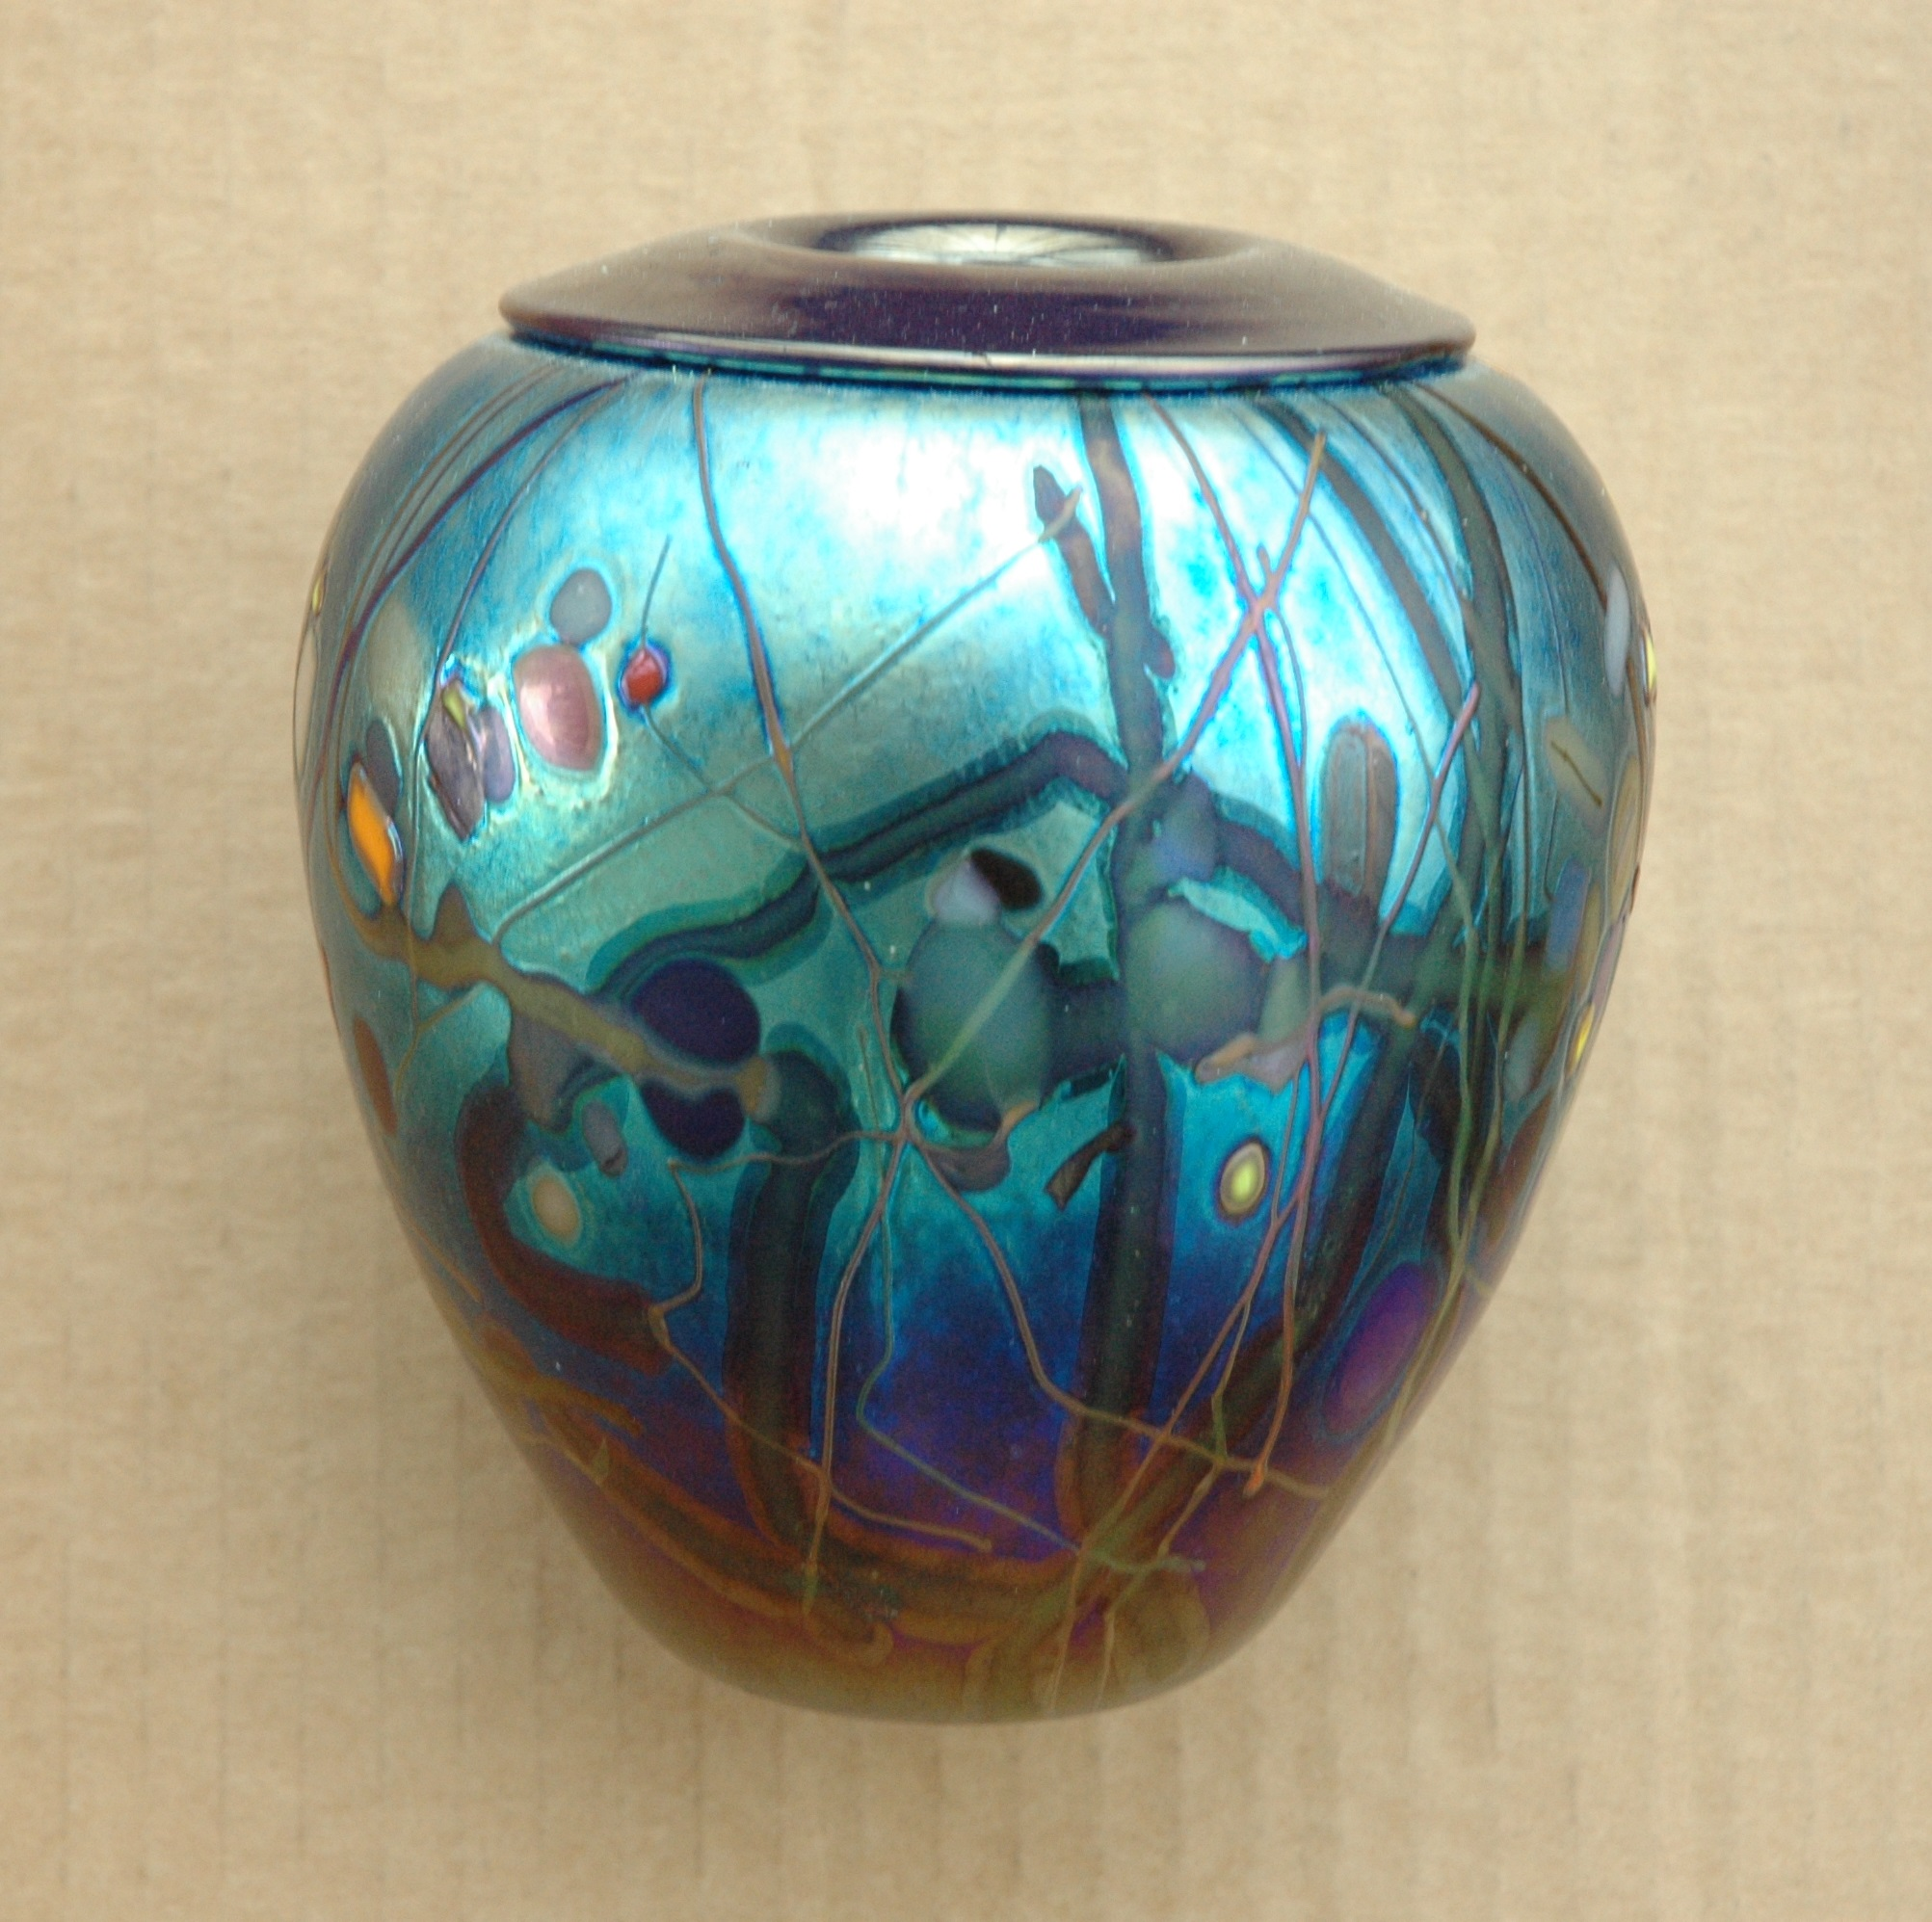
\includegraphics[width=0.2\textwidth]{img/interp/real_data/vase/vase.jpg}\\
  (a). Property settings & (b). Synthetic sphere & (c). Synthetic vase & (d). Real-world vase\\
\end{tabular}
\caption{The UI for determining the property settings, including albedo, specular, and roughness of the surface. As shown in (a), the problem condition in this case is: texture (0.8), albedo (0.8), specular (0.2), roughness(0.2). (b) demonstrates the effect of the property settings on a sphere, (c) on a teapot, and (d) shows the real-world object.}
\label{fig:prop_estimate}
\end{figure}

Now that we have proposed the model and representations of 3D reconstruction problem, we can express the four proposed problem conditions using this description. Given that all user perceived estimates would likely to be of low resolution, we use three discrete scales to set these properties: \textit{low} (0.2), \textit{medium} (0.5), and \textit{high} (0.8). The expression of the reconstruction problem is shown in table~\ref{tab:express}.
\begin{table}[!htbp]
  \centering
  \begin{tabular}{l*{4}{p{1cm}}l}
  \toprule
  \textbf{Object} & Texture & Albedo & Specular & Rough & \textbf{Label}\\
  \midrule
  Class 1 & low/med & high & low/med & high & Tl-B-D-R\\
  Class 2 & low/med & high & high & low/med & Tl-B-M-S\\
  Class 3 & high & high & low/med & high & T-B-D-R\\
  Class 4 & high & high & high & low/med & T-B-M-S\\
  \bottomrule
  \end{tabular}
  \caption{Expression of the reconstruction problem for the four problem conditions proposed in Section~\ref{ch:3DRecon_ProbSpace}.}
  \label{tab:express}
\end{table}

\section{Discussion and Conclusions}
This chapter builds upon the problem space proposed in Chapter~\ref{ch:3DRecon_ProbSpace}, and aims to provide a description to allow users to define problem condition of an object definitively. The description consists of two parts: a model and corresponding representations. The model answers the question of \textit{what} characteristic features of an object to describe, and the representations address the issue of \textit{how} to describe the selected set of features of an object.

We selected a subset of properties from the problem space as components of the model, and proposed corresponding representations for this model, as shown in Table~\ref{tab:3DRecon_model_repre}. We further analyze how easy it is to perceptually estimate properties, and express the four problem conditions using the proposed description. The proposed description is the first layer of our three-layer description-based interface. It works as the input of interpreter, and from which, an algorithm that works reliably will be chosen to reconstruct a successful digital shape.

Since we only explore a subset of problem space, the proposed model and representations may be insufficient to describe some classes of object, especially objects with translucent, transparent, or refractive surfaces. However, the application of the description to a broader domain is limited by the availability of existing techniques. As long as reliably algorithms have been developed, we can extend the current description to incorporate complex reflective and geometric properties.
